\section{Glossar}
For a better understanding of the explanations on the following pages, all used formula symbols have been summarized and explained here. Great care has been taken to assign each value to an unambiguous formula symbol.
\begin{figure}[H]
    \centering
    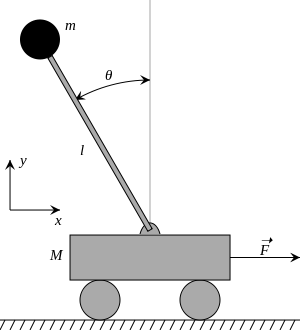
\includegraphics[width=0.4\textwidth]{Lab_report/pics/modelBuilding/300px-Cart-pendulum.svg.png}
    \caption{Sketch of the Balanbot}
    \label{fig:balanbot_sketch}
\end{figure}
% Please add the following required packages to your document preamble:
% \usepackage[table,xcdraw]{xcolor}
% If you use beamer only pass "xcolor=table" option, i.e. \documentclass[xcolor=table]{beamer}
\begin{table}[H]
\centering
\caption{Glossary }
\label{tab:glossary}
\begin{tabular}{|lx{1pt}l|l|}
\hline
\rowcolor[HTML]{C0C0C0} 
character      & description                                                                            & unit                     \\ \Xhline{1}
$x$            & Position of cart, may also be used as velocity: $\dot{x}$ and acceleration: $\ddot{x}$ & $m$,$^m/_s$, $^m/_{s^2}$ \\ \hline
$\Phi$         & pendulums position                                                                     & degree                   \\ \hline
$m_{cart}$     & Mass of the cart                                                                       & kg                       \\ \hline
$m_{pendulum}$ & Mass of the pendulum                                                                   & kg                       \\ \hline
$\mu$          & friction coefficient                                                                   & .                        \\ \hline
$I$            & moment of inertia                                                                      & $^m/_{s^2}$               \\ \hline
$F$            & Force generated by the motors acting in the movement direction                         & N                        \\ \hline
$F_x$          & Force in horizontal direction acting between pendulum and cart                         & N                        \\ \hline
$F_y$          & Force in vertical direction acting between pendulum and cart                           & N                        \\ \hline
$F_r$          & Friction force acting against the movement direction of the cart                       & N                        \\ \hline
$g$            & Gravitational Constant                                                                 & $^m/_{s^2}$               \\ \hline
$l$            & Length of pendulum                                                                     & $m$                      \\ \hline
$x_G$           &Distance in x-direction of the pendulum to the center of gravity of the system         &$m$                        \\ \hline
$y_G$           &Distance in y-direction of the pendulum to the center of gravity of the system         &$m$                        \\ \hline
$b$            &coefficient for F\textsubscript{r}                                                      & $\frac{kg}{s}$                      \\ \hline
\end{tabular}
\end{table}

\section{Model development}
The four base equations of the system have been derived from the sketch shown in \autoref{fig:forces}.

\begin{figure}[H]
    \centering
    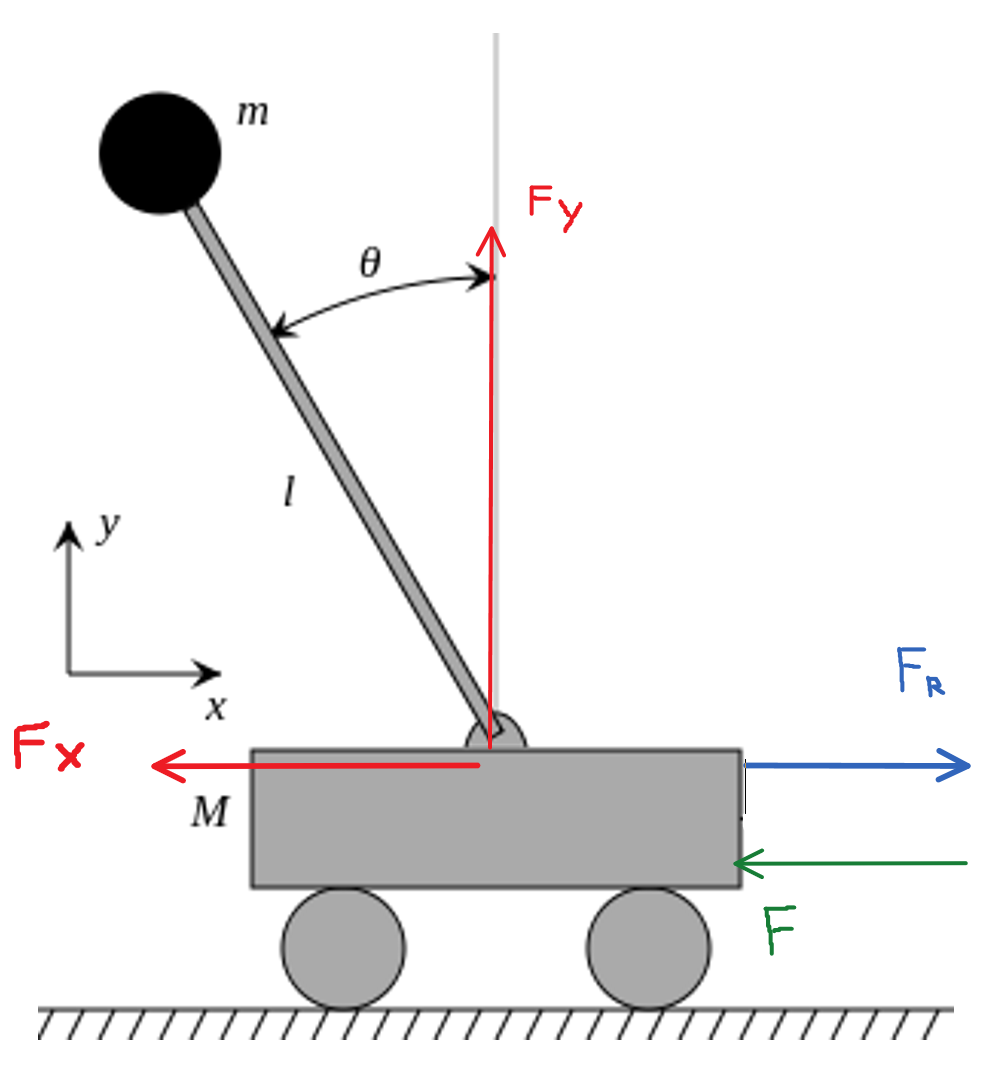
\includegraphics[width=0.4\textwidth]{Lab_report/pics/modelBuilding/forces.png}
    \caption{Sketch of the Balanbot, forces included}
    \label{fig:forces}
\end{figure}
\newpage
    \begin{align}    \label{eq: base 1 (a)}
        a = \ddot{x} = \frac{\sum F}{m_{cart}} = \frac{F-F_x-F_r}{m_{cart}}
    \end{align}

    \begin{align}    \label{eq: base 2 (alpha)}
            \ddot{\Theta} = \alpha = \frac{\sum T}{I} = \frac{F_x(cos(\Theta)-F_y sin(\Theta))}{I}
    \end{align}

    \begin{align}   \label{eq: base 3 (F_x)}
        F_x = m_{pendulum} \cdot \ddot{x_G} \notag\\
        x_G = x + l sin(\Theta)\notag \\
        \dot{x_G} = \dot{x} + l \dot{\Theta} cos(\Theta)\notag \\
        \ddot{x_G} = \ddot{x} - l \dot{\Theta} sin(\Theta) + l \ddot{\Theta} cos(\Theta)\notag \\ \cline{1-2}
        F_x = m_{pendulum}\cdot(\ddot{x} - l \dot{\Theta} sin(\Theta) + l \ddot{\Theta} cos(\Theta))
    \end{align}
 
    \begin{align}   \label{eq: base 4 (F_y)}
        F_y = m_{pendulum} \cdot (\ddot{y_G} + g)\notag \\
        y_G = l  cos(\Theta)\notag \\
        \dot{y_G} = -l  \dot{\Theta}  sin(\Theta)\notag \\
        \ddot{y_G} = -l \dot{\Theta}^2  cos(\Theta) - l \ddot{\Theta} sin(\Theta)\notag \\\cline{1-2}
        F_y = m_{pendulum} \cdot (g - l \dot{\Theta}^2  cos(\Theta) - l \ddot{\Theta} sin(\Theta))
    \end{align}
    After deriving the base equations from the system, the next goal is to merge the equations and receive final equations in the following form: $\ddot{x} = \dots$ and $\ddot{\Theta} = \dots$. The first final equation describes the acceleration of the system, the other one the angle of the pendulum. To receive this form, \autoref{eq: base 3 (F_x)} gets inserted into \autoref{eq: base 1 (a)}.
    
    \begin{align}\label{eq: final eq for x ddot}
        \ddot{x} \cdot m_{cart} = F-m_{pendulum}(\ddot{x}-l\dot{\Theta}^2 sin(\Theta)+l \ddot{\Theta} cos (\Theta))-\underbrace{b\dot{x}}_\text{F\textsubscript{r}})\notag \\
         \ddot{x} m_{cart} = F-m_{pendulum}\cdot\ddot{x}+m_{pendulum}l\dot{\Theta}^2 sin(\Theta)-m_{pendulum}l\ddot{\Theta}cos(\Theta)-b\dot{x}\notag \\
         \ddot{x}(m_{cart}+m_{pendulum})+b\dot{x}=F+m_{pendulum}l\dot{Phi}^2 sin(\Theta)-m_{pendulum}l\ddot{\Theta}cos(\Theta)\notag \\\notag \\\hline \notag \\
         \ddot{x} = \frac{F+m_{pendulum}l\dot{\Theta}^2 sin(\Theta)-m_{pendulum}l\ddot{\Theta}cos(\Theta)-b\dot{x}}{m_{cart}+m_{pendulum}}
    \end{align}
    \\
    To obtain $\ddot{\Theta} = \dots$, \autoref{eq: base 3 (F_x)} and \autoref{eq: base 4 (F_y)} get inserted into \autoref{eq: base 2 (alpha)}:
    \begin{align} \label{eq: final eq for Phi ddot}
        \ddot{\Theta} I = m_{pendulum} (\ddot{x} - l\dot{\Theta}^2 sin(\Theta) + l\ddot{\Theta} cos(\Theta))\cdot lcos(\Theta)-m_{pendulum}(g-l-\dot{\Theta}^2 cos(\Theta)-l\ddot{\Theta}sin(\Theta))\cdot l\sin(\Theta)\notag \\\notag\\
        \ddot{\Theta} I = m_{pendulum} l cos(\Theta) \ddot{x} \cancel{- m_{pendulum} l^2 cos(\Theta) sin(\Theta) \dot{\Theta}^2} + m_{pendulum} l^2 cos^2(\Theta) \ddot{\Theta} - m_{pendulum}g l sin(\Theta) \dots \notag\\ \dots \cancel{+m_{pendulum}l^2 sin(\Theta)cos(\Theta)\dot{\Theta}^2}+m_{pendulum}l^2 sin^2(\Theta)\ddot{\Theta}\notag \\\notag \\
        \ddot{\Theta} I = m_{pendulum} l cos(\Theta) \ddot{x} + m_{pendulum} l^2 \ddot{\Theta} (\underbrace{cos^2(\Theta)+sin^2(\Theta)}_\text{= 1})-m_{pendulum} g l sin(\Theta)\notag \\
         \ddot{\Theta} I + m_{pendulum}l^2\ddot{\Theta} = m l cos(\Theta)\ddot{x} + m_{pendulum} g l sin(\Theta)\notag \\\cline{1-2}\notag \\
         \ddot{\Theta} = \frac{m_{pendulum}\cdot lcos(\Theta)\ddot{x}+m_{pendulum}\cdot glsin(\Theta)}{I+m_{pendulum}\cdot l^2}
    \end{align}
\newpage
\subsection{Model of the System}
In this next step, the Model was transferred to MatLab Simulink and tested. For further use this model was saved as a submodel.
\begin{figure}[H]
    \centering
    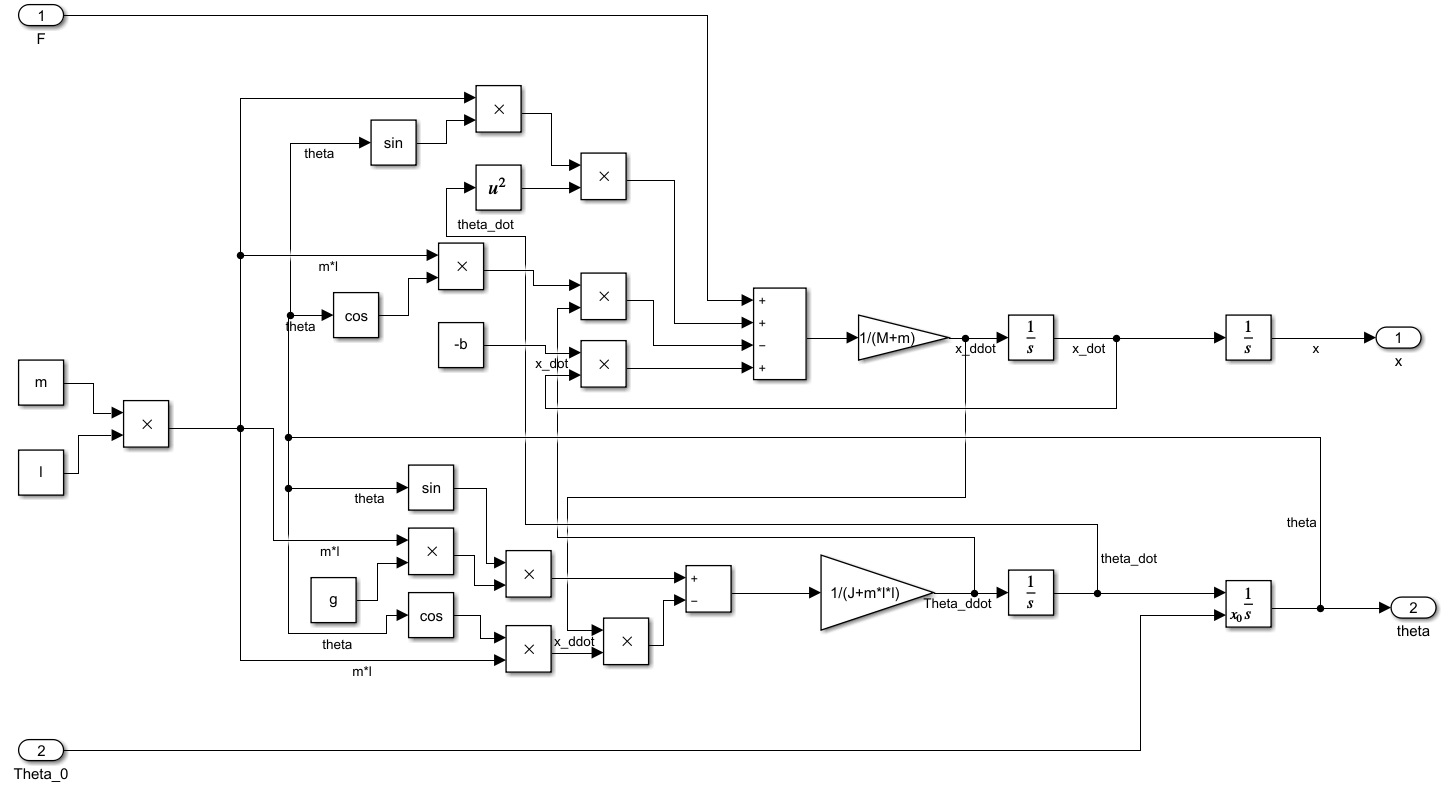
\includegraphics[width=1\textwidth]{Lab_report/pics/modelBuilding/non_linearized_model.PNG}
    \caption{Simulink Subsystem of non linearized model}
    \label{fig:non_linearized_model}
\end{figure}
\subsection{Analysis of the System}
\label{ssec:Analysis_of_non_lin_system}
\subsubsection{theta = 0}
The first part of analysis of our system was to test the behavior of the system when no force is put on the cart and the pendulum is completely upright when starting.

In the ``real world`` it would be expected that the pendulum will begin to fall in a considerably small time (maybe a few seconds of upright position). This may come from small air movements around the pendulum, an imprecise placement of the pendulum, or more relativistic effects (like the Brownian particle movement). 

However since these before mentioned interference weren't modeled in Simulink the pendulum should remain completely upright when simulating under these circumstances. 
\begin{figure}[H]
    \centering
    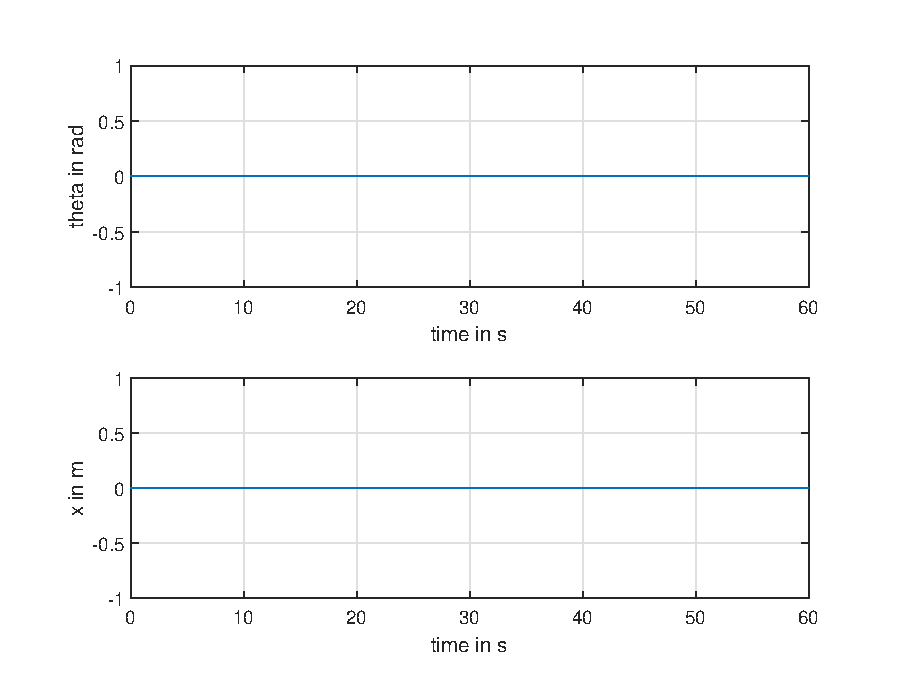
\includegraphics[width=0.8\textwidth]{Lab_report/pics/plots/non_linearized_results_theta_0.eps}
    \caption{Simulation results non-linearized model, $\Theta=0$}
    \label{fig:sim_res_non_lin_t_0}
\end{figure}

As can be seen in \autoref{fig:sim_res_non_lin_t_0}, the model behaves exactly as expected. The pendulum remains upright and the cart is not moving. For that matter: Complete success.

Be that as it may. The discussion about System Stability should nevertheless take place. Even if the results of this simulation suggest that the system might be stable, even the slightest action on the system will cause it to become unstable and not return to it's origin position. This leads to the conclusion, that an inverse Pendulum is not a stable system. 

\subsubsection{theta = 5}
The next step was to test the model with an initial angle of $\Theta=5^\circ$. In comparison to the last scenario now the pendulum should not remain upright, but should slowly begin to swing. Due to the simulated friction the amplitude of the swinging should decay by time.

\begin{figure}[H]
    \centering
    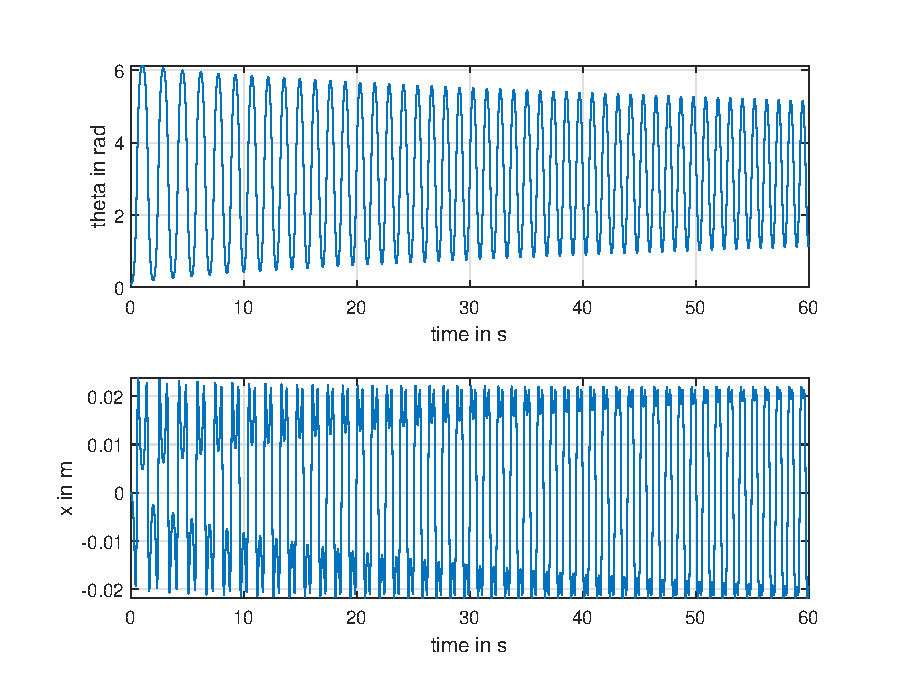
\includegraphics[width=0.8\textwidth]{Lab_report/pics/plots/non_linearized_results_theta_5.eps}
    \caption{Simulation results non-linearized model, $\Theta=5^\circ$}
    \label{fig:sim_res_non_lin_t_5}
\end{figure}
To make the amplitude decay even clearer, and to exclude all other causes of this decay, one more simulation was made. Now the factor for the friction was increased by a factor of 6, to result in $b=0.6$. All other parameters of the simulation remained the same. 
\begin{figure}[H]
    \centering
    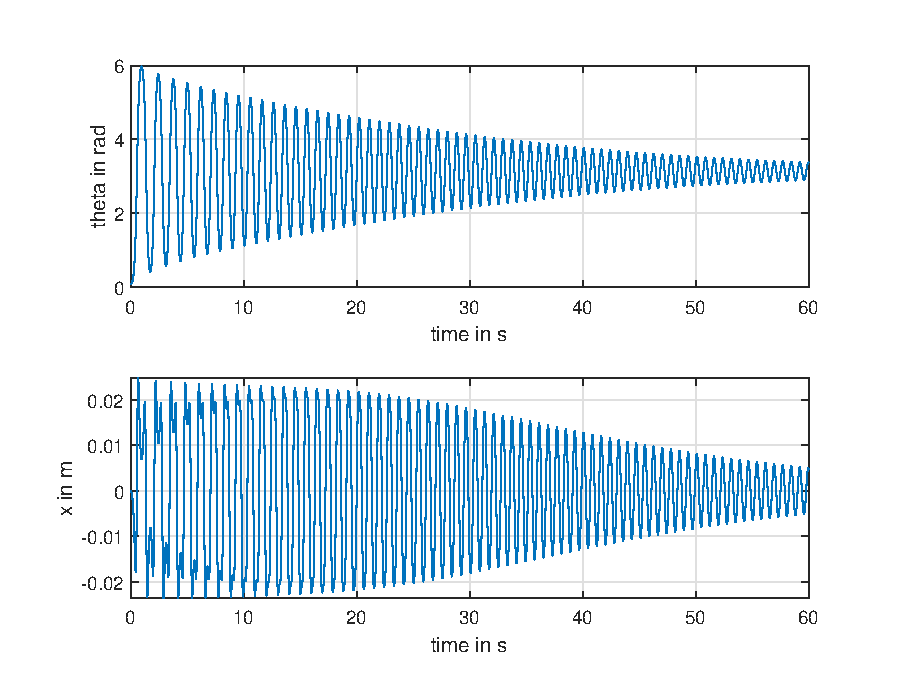
\includegraphics[width=0.8\textwidth]{Lab_report/pics/plots/non_linearized_results_inc_friction.eps}
    \caption{Simulation results non-linearized model, $\Theta=5^\circ$}
    \label{fig:sim_res_non_lin_t_5_inc_fric}
\end{figure}
The increased rate of decay can be observed very clearly in \autoref{fig:sim_res_non_lin_t_5_inc_fric}.

As already discussed in the previous section, this is an unstable system. However the implications of that term can be seen a lot easier during the simulations results shown in \autoref{fig:sim_res_non_lin_t_5} and \autoref{fig:sim_res_non_lin_t_5_inc_fric}. In the Plot which shows the angle of the pendulum it can be seen, that the system, when excited will not return to its original position (which would be $\Theta=0$), but in its normal (not inverse) pendulum position ($\Theta = 180^\circ =\pi \text{ rad}$).
\section{Linearization}
To explain the step of Linearization our first step is to show which parts of our function are not linear. According to an general definition of Linearity, linearity describes the property of a system to always respond to a change in one parameter with a proportional change in another parameter (\cite{dewiki:Linearity}). This is not true for sine and cosine functions. These are not linear. Per se this isn't a problem, but it can make some future steps and simulations a lot easier if these function were replaced by a different expression.

A general approach to linearising these functions is the development of a Taylor Polynom with varying degree (The higher the degree of the Polynome, the preciser the approximation). In our specific case we have the added bonus of only using very small angles. When looking closely at the course of the function (\autoref{fig:sine_cos}), it can be seen that the sine and cosine functions at very low angles can also be calculated without the development of a Taylor series (better: only using the first term of the Taylor series) to estimate the value. The error resulting of this process will be discussed in a future chapter(see \autoref{ssection:Comparison_lin_non_lin}).
\begin{figure}[H]
    \centering
    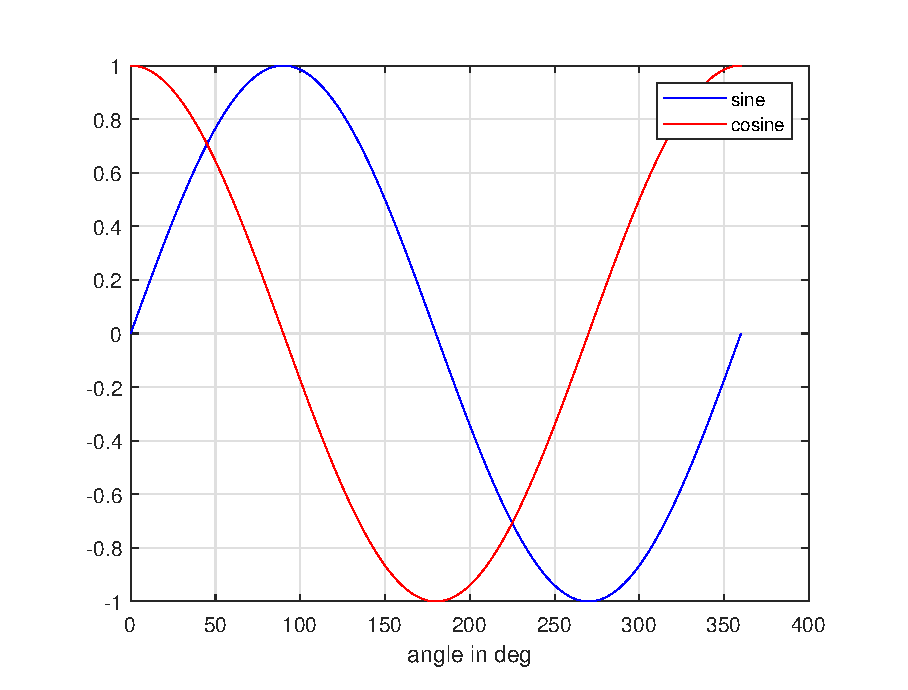
\includegraphics[width=0.8\textwidth]{Lab_report/pics/plots/sin_cos.eps}
    \caption{plot of sine and cosine}
    \label{fig:sine_cos}
\end{figure}
\subsection{Excursus Taylorseries}
To further explain how the before mentioned non-linear functions can be replaced, the Taylor Series will be developed for both. The general definition of the Taylor Series is:
\begin{equation}
      T_{f(x;a)} = \sum^\infty_{n=0} \frac{f^{(n)}(a)}{n!}(x-a)^n
    \label{eq:Taylor_Series}  
\end{equation}
\subsubsection{Sine Function}
To get the corresponding values for the Linerization it was decided to get the developed Taylor series from a collection of formulas(\cite{papula2017mathematische}).
\begin{align}
    \sin \,(x)&=\sum _{n=0}^{\infty }(-1)^{n}{\frac {x^{2n+1}}{(2n+1)!}} \\
    &=x-{\frac {x^{3}}{6}}+{\frac {x^{5}}{120}}-\cdots \cite[p. 187]{papula2017mathematische}
\end{align}
Since the development of the series stops at the first term, the linearized version of the $\sin(x)$ is $x$.
\subsubsection{Cosine Funktion}
\begin{align}
    cos(x)&=\sum _{n=0}^{\infty }(-1)^{n}{\frac {x^{2n}}{(2n)!}}\\
    &=1-{\frac {x^{2}}{2}}+{\frac {x^{4}}{24}}-\cdots  \cite[p. 187]{papula2017mathematische}
\end{align}

Since the development of the series stops at the first term, the linearized version of the $\cos(x)$ is $1$.
\newpage
\subsection{Simulink Model}
The linearization of the before developed MatLab model is a fast and easy step. In that our case we just replaced the sine and cosine Blocks with the corresponding gains. 
\begin{figure}[H]
    \centering
    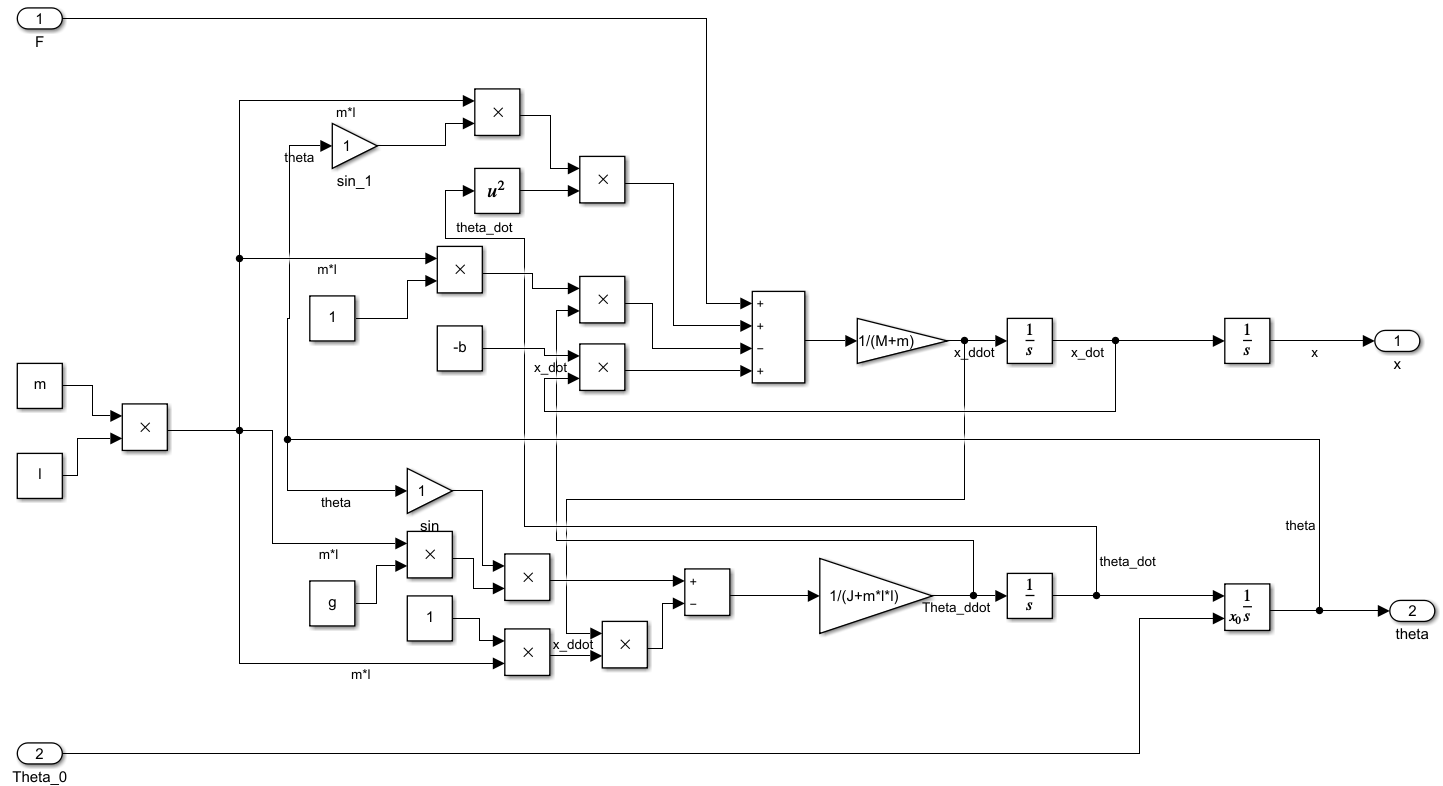
\includegraphics[width=\textwidth]{Lab_report/pics/modelBuilding/linearized_model.PNG}
    \caption{linearized model}
    \label{fig:lin_model}
\end{figure}
\subsection{Analysis of the System}
In an ideal case the resulting values would look the same as in the non-linearized Version (see \autoref{ssec:Analysis_of_non_lin_system}). However, since we already saw angles which are bigger than the $\pm 5^\circ$ which were specified during the linearization process the results can and will differ greatly from the non-linear results.
\begin{figure}[H]
    \centering
    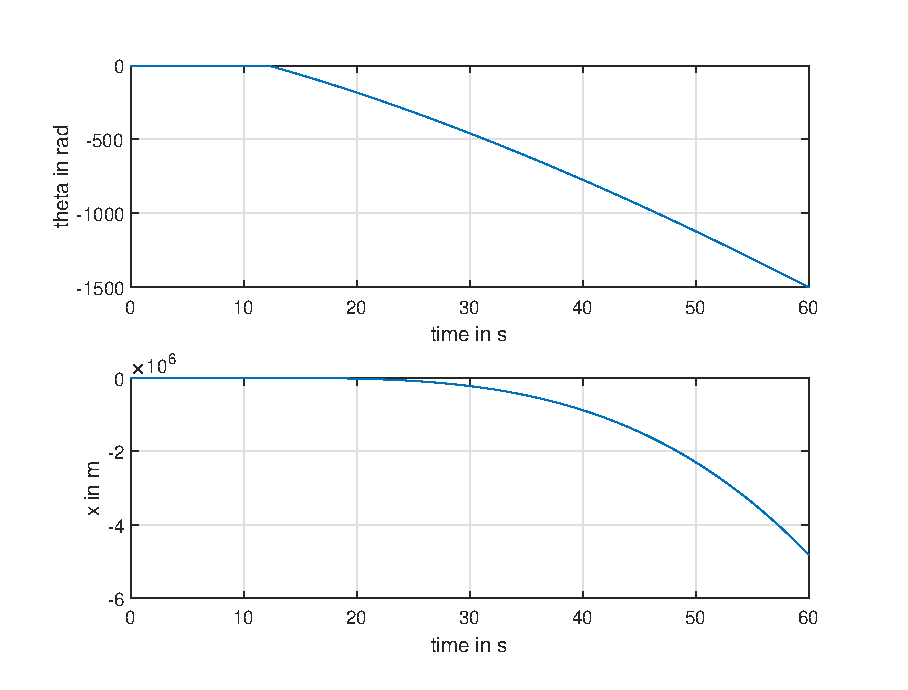
\includegraphics[width=0.8\textwidth]{Lab_report/pics/plots/linearized_results_theta_0.eps}
    \caption{Simulation results linearized model, $\Theta=0^\circ$}
    \label{fig:sim_res_non_lin_t_5}
\end{figure}
\begin{figure}[H]
    \centering
    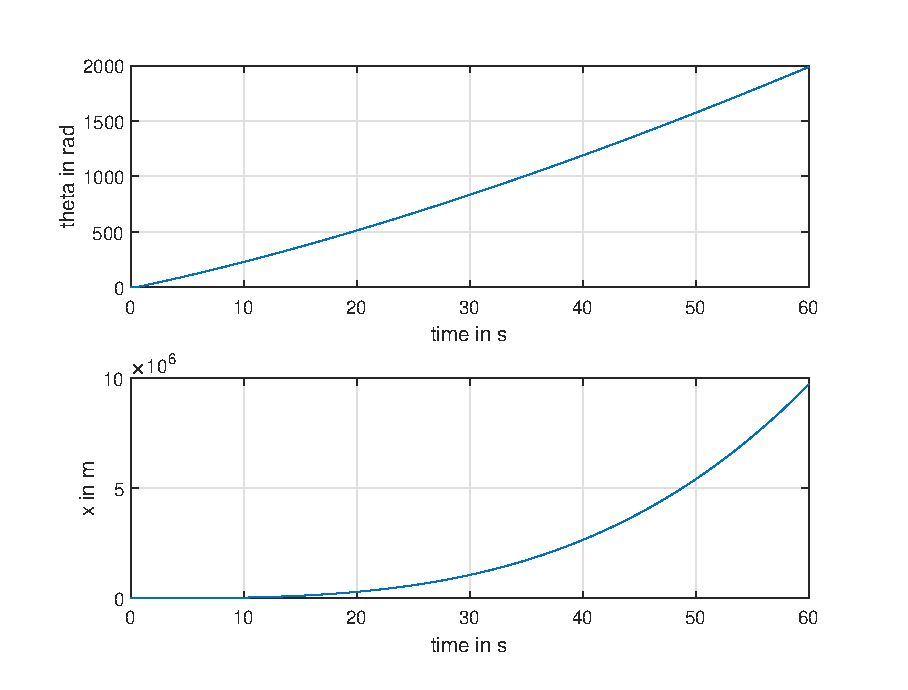
\includegraphics[width=0.8\textwidth]{Lab_report/pics/plots/linearized_results_theta_5.eps}
    \caption{Simulation results linearized model, $\Theta=5^\circ$}
    \label{fig:sim_res_non_lin_t_5}
\end{figure}
\section{Comparison of linear vs. non-linear System}
\label{ssection:Comparison_lin_non_lin}
As expected were the results of linearized system not as stable and in every case not as reliable as the results of the non-linear system. The Results can surely be improved by using more than one Term of the Taylor series (i.e. 8-10), however this would lead to increased system complexity. One other factor of the linearized system is, that the results are a better use for short simulation times and thus probably good enough for the development of the controller. 

\section{System Analysis with Transfer Function}
%%Fabi have fun
Open loop response with no offset
Open loop response with initial condition $\Theta = 5^\circ$
\begin{align}\label{eq: 1}
        cos(\Theta)=cos(\phi+\pi)\xrightarrow{\phi\rightarrow0}-1\\
        sin(\Theta)=cos(\phi+\pi)\xrightarrow{\phi\rightarrow0}-\phi\\
        \dot{\Theta}=\frac{d(\phi+\pi)}{dt}=\dot{\phi}=0
\end{align}

\begin{align}\label{eq: 1}
        \RN{1}:\ddot{x} = [F+ml\ddot{\Theta}-y_{1}\dot{x}] \frac{1}{(M+m)}\\
        \RN{2}:\ddot{\Theta} = [-mgl\Theta+ml\ddot{x}] \frac{1}{(J+ml^2)} 
    \end{align}
\begin{align}\label{eq: 2}
        \Theta s^2=\frac{1}{(J+ml^2)}[-mgl\Theta+mlxs^2]\\
        (J+ml^2)\Theta s^2+mgl\Theta=mlxs^2\\
        \Theta[s^2(J+ml^2)+mgl]=mlxs^2\\
        \Theta=\frac{mlxs^2}{s^2(J+ml^2)+mgl}
    \end{align}
\begin{align}\label{eq: 3}
            (M+m)xs^2+y_{1}xs=F+ml\Theta s^2\\
        x[s^2(M+m)+sy_{1}]=F+s^2ml\Theta
    \end{align}
\begin{align}\label{eq: 4}
        x[s^2(M+m)+sy_{1}]=F+s^2ml\frac{mlxs^2}{s^2(J+ml^2)+mgl}\\
        x[s^2(M+m)+sy_{1}-\frac{m^2l^2s^4}{s^2(J+ml^2)+mgl}=F\\
        \frac{x}{F}=\frac{1}{\frac{[s^2(M+m)+y_{1}s][s^2(s+ml^2)+mlg]-(m^2l^2s^4)}{s^2(J+ml^2)+mlg}}\\
        \frac{x(s)}{F(s)}=\frac{s^2(J+ml^2)-mlg}{s^4[(M+m)(J+ml^2)-m^2l^2]+s^3[y_{1}(J+ml^2)]-s^2[(M+m)mlg]-s[y_{1}mlg]}
    \end{align}
\begin{align}\label{eq: 5}
        x[s^2(M+m)+sy_{1}]=F+s^2ml\frac{mlxs^2}{s^2(J+ml^2)+mgl}\\
        x[s^2(M+m)+sy_{1}-\frac{m^2l^2s^4}{s^2(J+ml^2)+mgl}=F\\
        \frac{x}{F}=\frac{1}{\frac{[s^2(M+m)+y_{1}s][s^2(s+ml^2)+mlg]-(m^2l^2s^4)}{s^2(J+ml^2)+mlg}}\\
        \frac{\Theta(s)}{F(s)}=\frac{s^2(ml)}{s^4[(M+m)(J+ml^2)-m^2l^2]+s^3[y_{1}(J+ml^2)]-s^2[(M+m)mlg]-s[y_{1}mlg]}
    \end{align}